\documentclass[UTF8]{ctexart}
\usepackage{amsmath}
\usepackage{float}
\usepackage{indentfirst}
\usepackage{listings}
\usepackage{xcolor}
\lstset{
    %backgroundcolor=\color{red!50!green!50!blue!50},%代码块背景色为浅灰色
    rulesepcolor= \color{gray}, %代码块边框颜色
    breaklines=true,  %代码过长则换行
    numbers=left, %行号在左侧显示
    numberstyle= \small,%行号字体
    %keywordstyle= \color{red},%关键字颜色
    %commentstyle=\color{green!90}, %注释颜色
    frame=shadowbox%用方框框住代码块
    }
\usepackage{graphicx}
\usepackage[a4paper, left = 3.17cm, right = 3.17cm, top=2.54cm, bottom=2.54cm]{geometry}
\setlength{\parindent}{2em}
\title{第二讲-习题}
\author{姜帆}
\date{\today}
\begin{document}
\maketitle
\tableofcontents
\newpage
\section{基础作业}
\subsection{Allen方差标定}
\subsubsection{Allen方差标定原理简述}
\indent 目前,常用的随机误差识别方法包括功率谱密度(PSD)、自相关函数估计、AIlan方差估计等方法。A11an方差分析法最初是1966年由美国国家
标准局的David Allan为了研究原子钟的振荡器的稳定性而提出的,这种方法因其可以克服标准差对包含调频闪变噪声时出现的发散而得到广
泛的应用。1980年,Allan方差被引入到陀螺仪的随机误差识别中,之后主要在中、低精度激光和光纤陀螺信号性能分析中使用。由于该方法的实用
性强1998年A1lan方差被IEEE协会选为分析光纤陀螺随机误差的推荐方法。在2003年Allan方差第一次被应用到MEMS陀螺仪随机误差的分
析中,并取得了预期的识别效果。由于陀螺等惯性传感器本身也具有振荡器的特征,因此该方法随后被广泛应用于各种惯性传感器的随机误差辨识中。\\
\indent A11an方差是一种基于时域的分析方法,它的特点是不仅能够确定产生数据噪声的基本随机过程的特性,而且能够识别给定噪声项的来源。它能
非常容易地对误差源以及对整个噪声特性的影响程度进行细致的表征和识别,计算方便,易于分离。\\
\indent A11an方差是一种从时域上对信号频域稳定性进行分析的通用方法,也就是将随机误差作为时间序列来处理,描述其均方误差的方法。设一定的采样时间间隔
对数据集进行采样,把所获数据进行分组;对每个子集求平均值;对每个不同平均时间计算A11an方差;作出A11an标准差随平均时间变化的双对数曲线。\\
\begin{figure}[H]
\centering
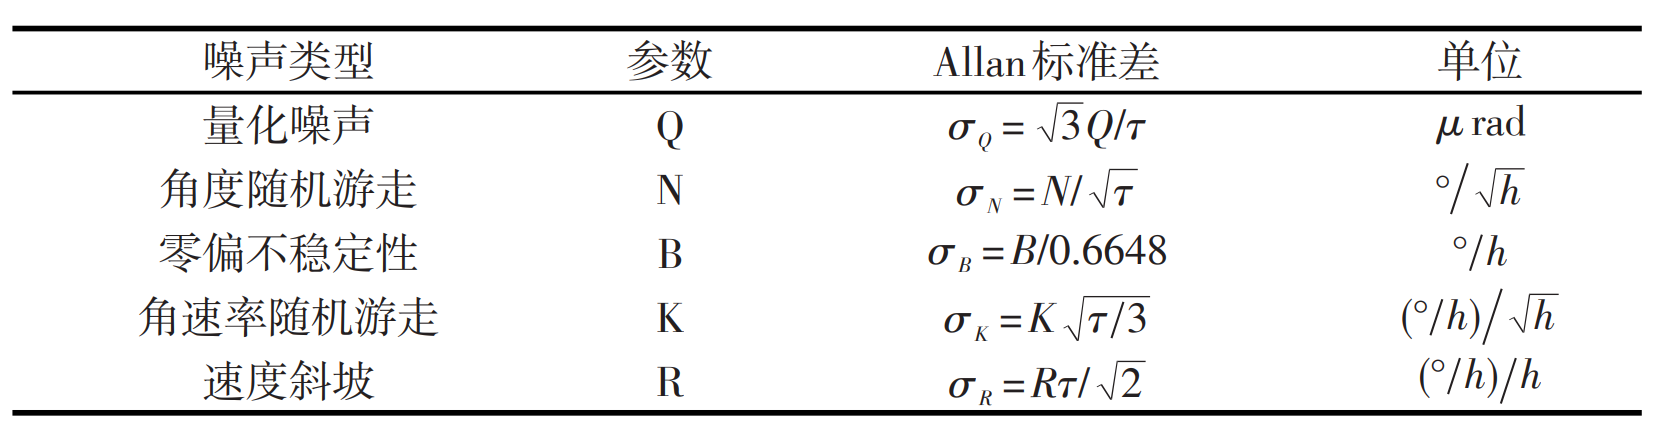
\includegraphics[width=0.9\textwidth]{allen1.png}    
\caption{Allan方差与常见噪声对应关系}
\label{img0}
\end{figure}
\begin{figure}[H]
\centering
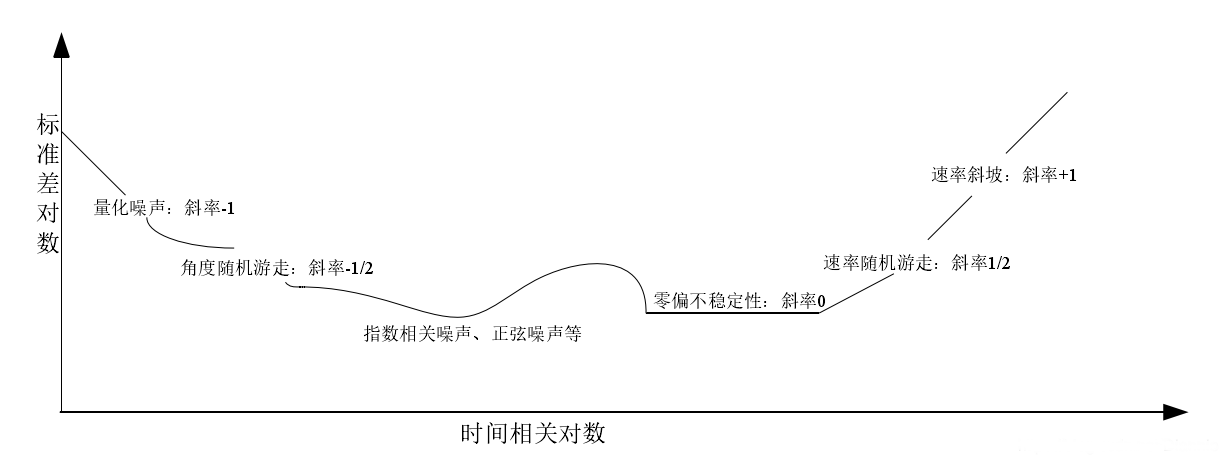
\includegraphics[width=0.9\textwidth]{allen2.png}    
\caption{Allan曲线示意图}
\label{img0}
\end{figure}
\subsubsection{Allen方差标定实验}
\indent 本文实验使用imu\_utils工具生成allan曲线。\\
\indent 实验流程为:\\
\indent (1)进入ros工作空间,配置vio\_data\_simulation功能包,并运行生成imu.bag文件。\\
\indent\indent rosrun vio\_data\_simulation vio\_data\_simulation\_node\\
\indent (2)进入ros工作空间,配置imu\_utils功能包。回放imu.bag文件。同时运行imu\_utils。\\
\indent\indent roslaunch imu\_utils simulation.launch\\
\indent\indent rosbag play -r 200 ../src/vio\_data\_simulation/data/imu2.bag\\
\indent (3)画出Allan曲线\\
\indent 下面为曲线绘制脚本\\
\begin{lstlisting}[language={matlab}]
    clear 
    close all
    
    dt = dlmread('../data/data_simulation_imu2_gyr_t.txt');         
    data_x = dlmread('../data/data_simulation_imu2_gyr_x.txt'); 
    data_y= dlmread('../data/data_simulation_imu2_gyr_y.txt'); 
    data_z = dlmread('../data/data_simulation_imu2_gyr_z.txt'); 
    data_drawavg=(data_x +data_y +data_z)/3/3600*(2.*3.141593653)/360;
    data_draw=[data_x data_y data_z]/3600*(2.*3.141593653)/360 ;
    data_sim_x= dlmread('../data/data_simulation_imu_sim_gyr_x.txt'); 
    data_sim_y= dlmread('../data/data_simulation_imu_sim_gyr_y.txt'); 
    data_sim_z= dlmread('../data/data_simulation_imu_sim_gyr_z.txt'); 
    data_sim_draw=[data_sim_x data_sim_y data_sim_z]/3600*(2*3.141593653)/360 ;
    figure(1)
    loglog(dt, data_draw(:,1) , 'r+');
    hold on;  
    loglog(dt, data_draw(:,2) , 'b+');
    hold on;  
    loglog(dt, data_draw(:,3) , 'k+');
    hold on 
    loglog(dt, data_drawavg , '-');
    legend('w_x','w_y','w_z','w_{avg}')
    mix_where=find(dt==1);
    num=dt(mix_where);
    xlabel('time:sec');                
    ylabel('Sigma:deg/h');   
    grid on;                           
    hold on;  
    %loglog(dt, data_sim_draw , 'r-');
    
    dt = dlmread('../data/data_simulation_imu_acc_t.txt');         
    data_x = dlmread('../data/data_simulation_imu2_acc_x.txt'); 
    data_y = dlmread('../data/data_simulation_imu2_acc_y.txt'); 
    data_z = dlmread('../data/data_simulation_imu2_acc_z.txt'); 
    data_draw=[data_x data_y data_z] ;
    data_draw_avg=(data_x +data_y +data_z)/3 ;
    data_sim_x= dlmread('../data/data_simulation_imu2_sim_acc_x.txt'); 
    data_sim_y= dlmread('../data/data_simulation_imu2_sim_acc_y.txt'); 
    data_sim_z= dlmread('../data/data_simulation_imu2_sim_acc_z.txt'); 
    data_sim_draw=[data_sim_x data_sim_y data_sim_z] ;
    figure(2)
    loglog(dt, data_draw(:,1) , 'r+');
    hold on
    loglog(dt, data_draw(:,2) , 'b+');
    hold on
    loglog(dt, data_draw(:,3) , 'k+');
    hold on
    loglog(dt, data_draw_avg, '-');
    legend('acc_x','acc_y','acc_z','acc_{avg}')
    ylabel('Sigma:m/s2');   
    xlabel('time:sec');   
    hold on
    % loglog(dt, data_sim_draw , 'b-');
    grid on;
\end{lstlisting}
1.第一组\\
\indent 连续时间的加速度的高斯白噪声方差设定为 0.019,连续时间的陀螺仪的高斯白噪声为 0.015。 连续时间的加速度 bias 的随机游走噪声设定为
5e−4 ,连续时间的陀螺仪的 bias 随机游走噪声设定为 5e−5。\\
\begin{figure}[H]
\centering
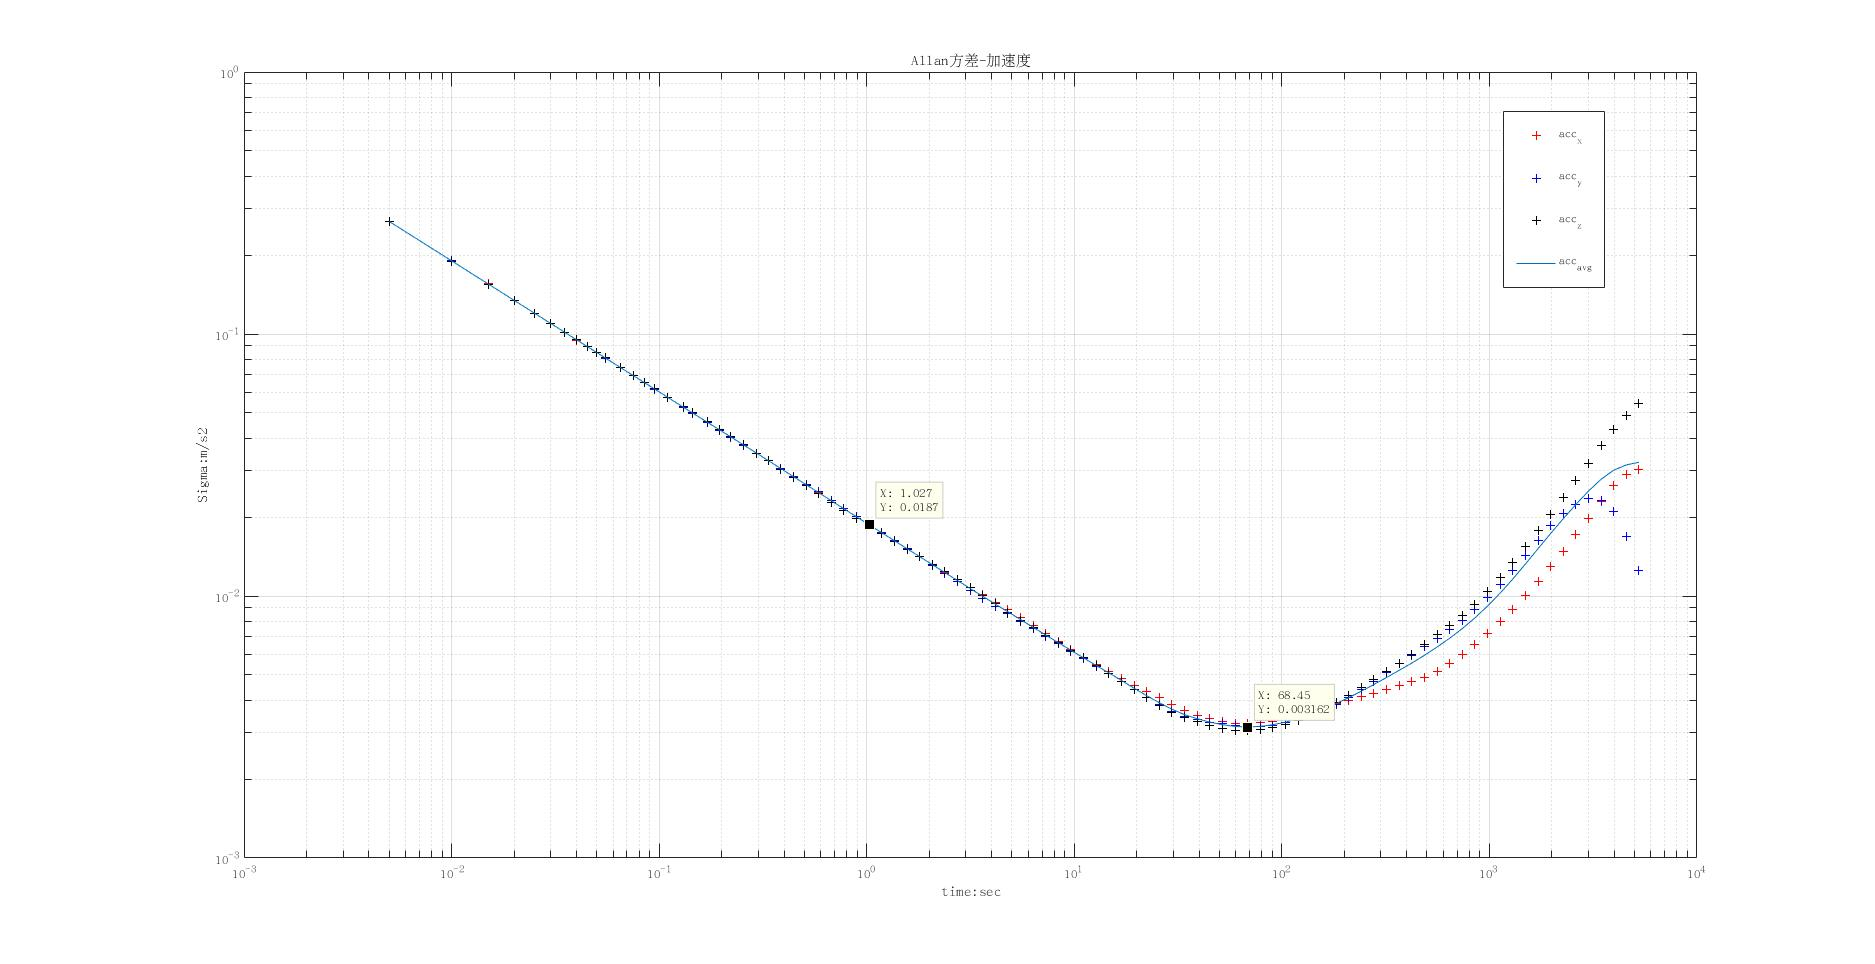
\includegraphics[width=1\textwidth]{acc_allan.jpg}    
\caption{连续时间的Allan方差-加速度}
\label{img0}
\end{figure}
\begin{figure}[H]
\centering
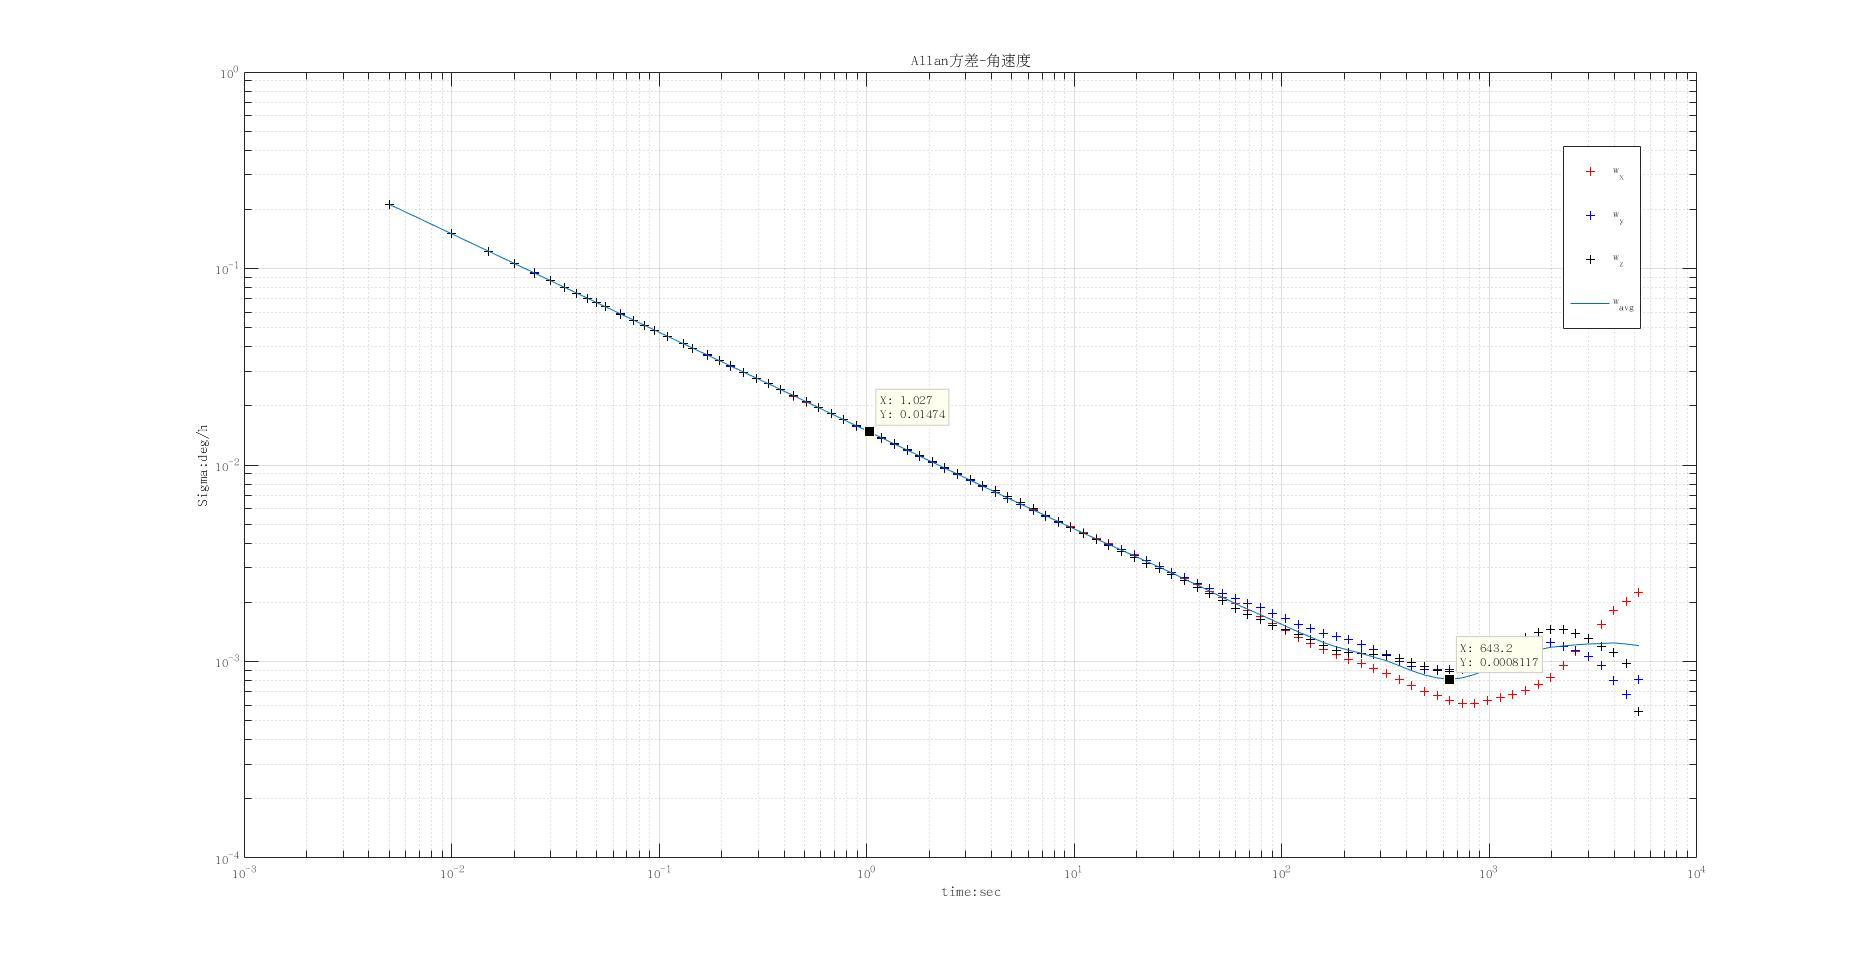
\includegraphics[width=1\textwidth]{gyo_allan.jpg}    
\caption{连续时间的Allan方差-角速度}
\label{img1}
\end{figure}
\indent 如图,绘制了IMU连续时间的加速度和角速度误差Allan方差曲线。从图中可以看出连续时间的加速度三个轴的平均值白噪声标定结果为0.0187,连续时间的加速度三个轴的平均值bias随机游走
噪声为3.1e-3;连续时间的角速度三个轴的平均值白噪声标定结果为0.147,连续时间的角速度三个轴的平均值bias噪声为8.1e-4。\\
2.第二组\\
\indent 连续时间的加速度的高斯白噪声设定为 0.035,连续时间的陀螺仪的高斯白噪声为 0.025。连续时间的加速度 bias 的随机游走噪声设定为
2e−3 ,连续时间的陀螺仪的 bias 随机游走噪声设定为 2e−4。\\
\begin{figure}[H]
\centering
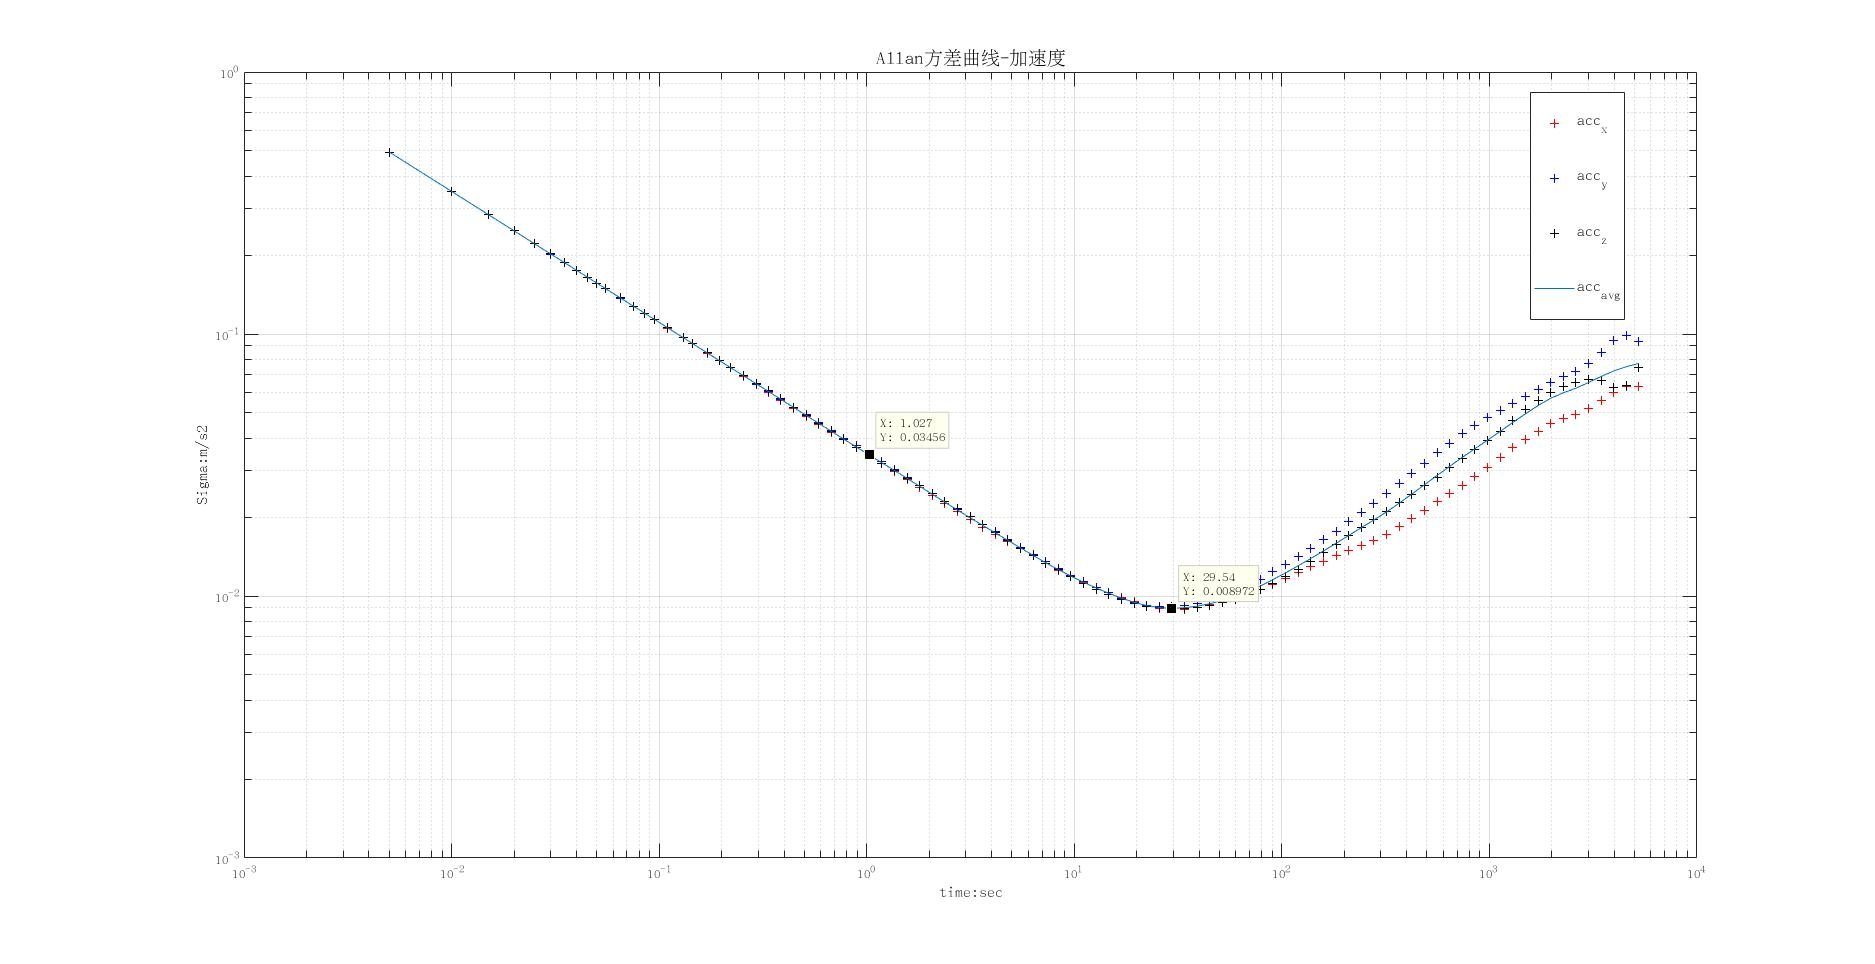
\includegraphics[width=1\textwidth]{acc_allan2.jpg}    
\caption{连续时间Allan方差-加速度}
\label{img0}
\end{figure}
\begin{figure}[H]
\centering
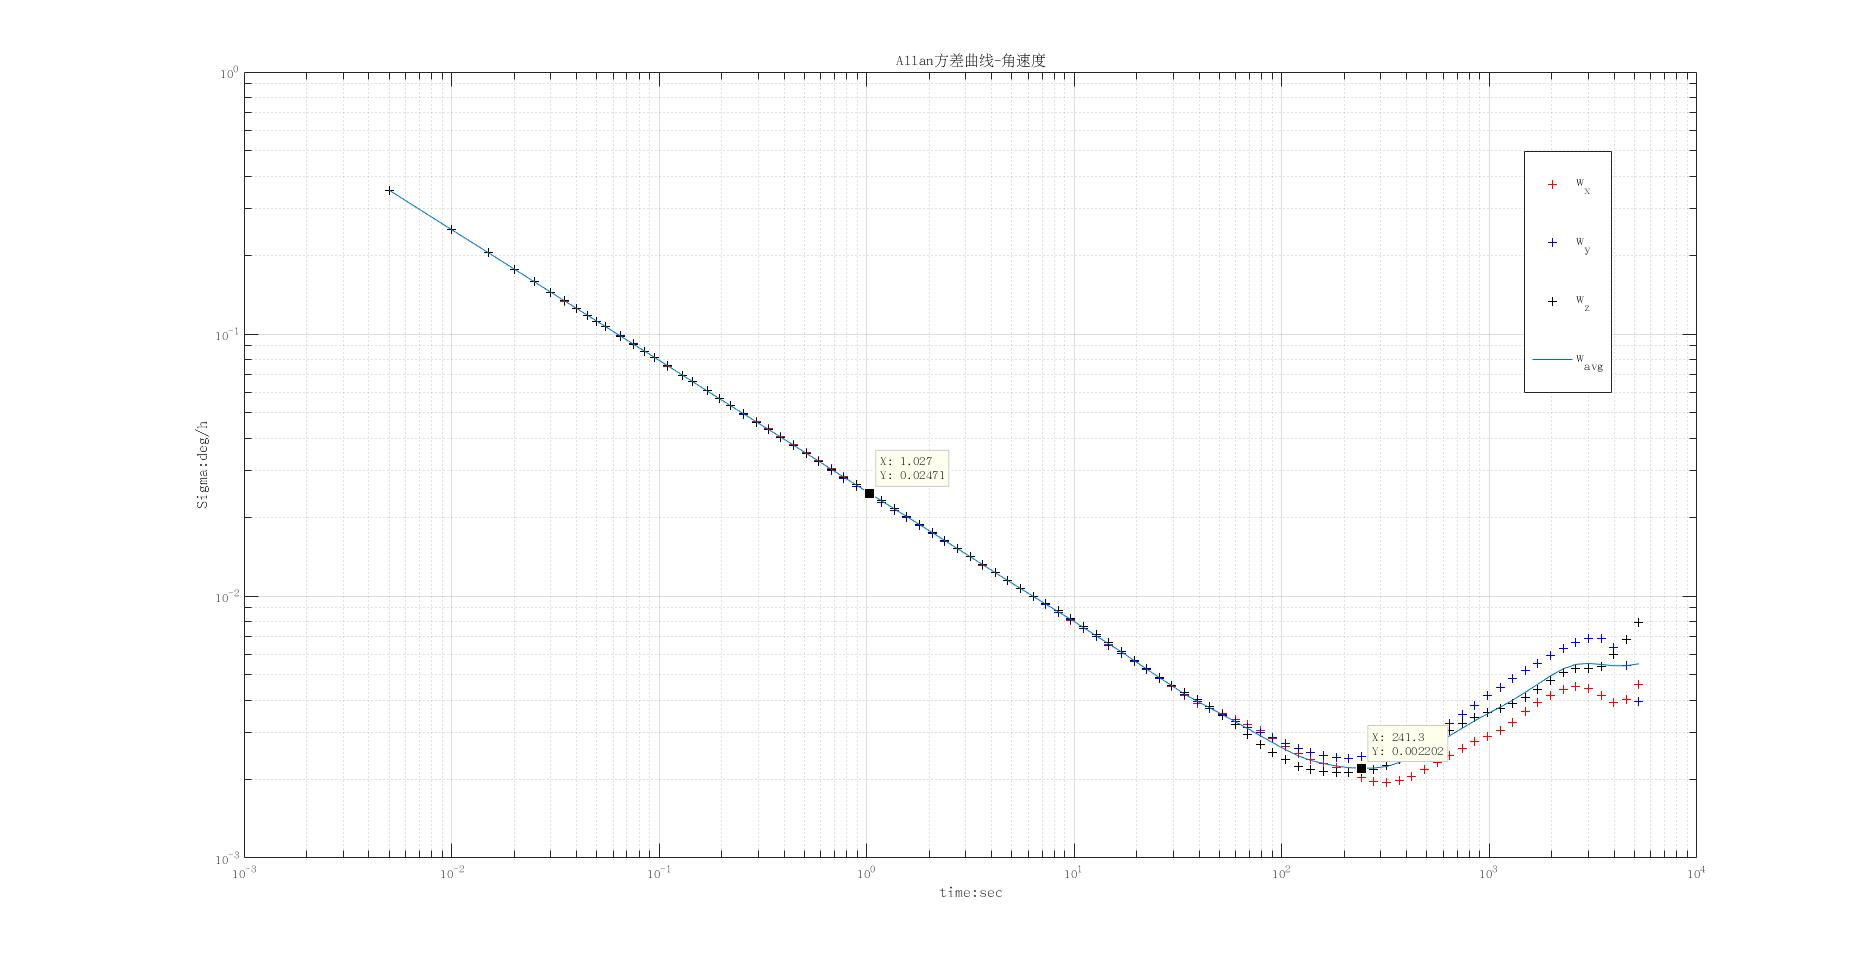
\includegraphics[width=1\textwidth]{gyo_allan2.jpg}    
\caption{连续时间的Allan方差-角速度}
\label{img1}
\end{figure}
\indent 如图,绘制了IMU连续时间的加速度和角速度误差Allan方差曲线。从图中可以看出连续时间的加速度三个轴的平均值白噪声标定结果为0.0345,连续时间的加速度三个轴的平均值bias随机游走
噪声为8.9e-3;连续时间的角速度三个轴的平均值白噪声标定结果为0.247,连续时间的角速度三个轴的平均值bias噪声为2.2e-3。\\
\indent 根据两次实验结果,可以发现Allan曲线标定的加速度高斯白噪声,角速度高斯白噪声与预设的基本吻合,但是加速度角速度bias随机
游走标定结果与预设差一个数量级。\\


\subsection{中值积分}
\indent 程序如下:\\
\begin{lstlisting}[language={c++}]
    double dt = param_.imu_timestep;
    Eigen::Vector3d Pwb = init_twb_;              // position :    from  imu measurements
    Eigen::Quaterniond Qwb(init_Rwb_);            // quaterniond:  from imu measurements
    Eigen::Vector3d Vw = init_velocity_;          // velocity  :   from imu measurements
    Eigen::Vector3d gw(0,0,-9.81);    // ENU frame
    Eigen::Vector3d temp_a;
    Eigen::Vector3d theta;
    for (int i = 1; i < imudata.size(); ++i) {

        /// 中值积分
        MotionData imupose = imudata[i];
        MotionData imuposenext = imudata[i-1];
        Eigen::Vector3d imu_gyro_mid = (imupose.imu_gyro + imuposenext.imu_gyro) / 2.0;       //w=1/2(wk-wk_biase+wk+1-wk+1_bias)
        Eigen::Quaterniond dq;
        Eigen::Vector3d dtheta_half = imu_gyro_mid * dt /2.0;
        dq.w() = 1;
        dq.x() = dtheta_half.x();
        dq.y() = dtheta_half.y();
        dq.z() = dtheta_half.z();
        Eigen::Quaterniond Qwbnext= Qwb * dq;             // qk+1=qk*deltaq
        Qwbnext=Qwbnext.normalized();
        Eigen::Vector3d acc_w = ((Qwb*(imupose.imu_acc)+gw) + (Qwbnext*(imuposenext.imu_acc)+gw)) /2.0;    //aw = ((Rkwb * ( acck_body - acck_bias ) + gw)+(Rk+1wb * ( acck+!_body - acck+1_bias ) + gw))/2
        Qwb = Qwbnext;
        Vw = Vw + acc_w * dt;
        Pwb = Pwb + Vw * dt + dt * dt * acc_w /2.0;


    }
\end{lstlisting}
\indent 下面为欧拉积分与中值积分得到的轨迹图:
\begin{figure}[H]
\centering
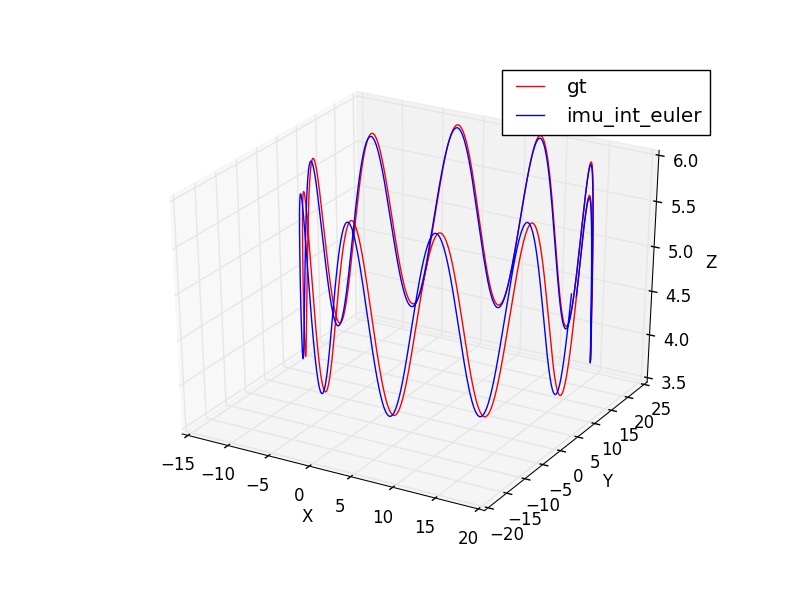
\includegraphics[width=0.8\textwidth]{euler.jpg}    
\caption{欧拉积分结果}
\label{img0}
\end{figure}
\begin{figure}[H]
\centering
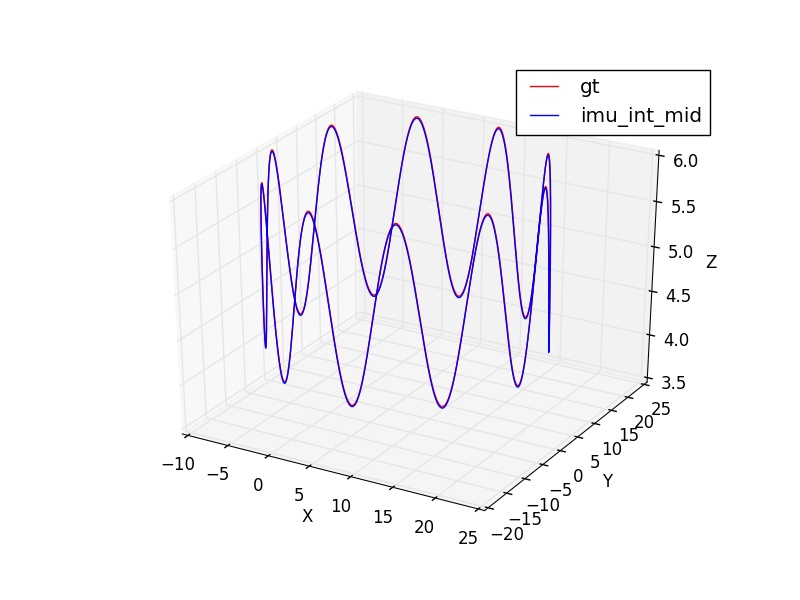
\includegraphics[width=0.8\textwidth]{mid.jpg}    
\caption{中值积分结果}
\label{img1}
\end{figure}
\indent 定性来看,由欧拉积分结果与中值积分结果图对比,我们可以看出IMU中值积分的结果比欧拉积分结果更加准确,
更加接近真值。\\
\indent 定量来看,通过计算得到欧拉积分结果与真值的均方根误差为0.00481,中值积分结果与真值的均方根误差为0.00070,因此IMU
中值积分结果要好于欧拉积分的结果

\newpage
\section{提升作业}
\indent 利用B样条曲线可以对已有轨迹仿真IMU数据。\\
\subsection{B样条曲线简介}
\indent 贝塞尔曲线于1962,由法国工程师皮埃尔·贝塞尔(Pierre Bézier)所广泛发表,他运用贝塞尔曲线来为汽车的主
体进行设计。贝塞尔曲线最初由Paul de Casteljau于1959年运用de Casteljau演算法开发,以稳定数值的方法求出贝塞尔曲线。
但是贝塞尔曲线存在一些问题:缺乏局部修改性;幂次太高难以修改;n 较大时,特征多边形的边数较多,对曲线的控制减弱。\\
\indent 1972年Riesenfeld提出了B样条曲线,用B样条基函数代替了贝塞尔曲线中的Bernstein基函数。\\
\indent 设有控制顶点$p_0,p_1,…,p_n$,则$k$阶$(k-1次)$B样条曲线的数学表达式为:\\
\begin{equation}
\begin{aligned}
p(t)=\sum_{i=1}^np_iB_{i,k}(t)
\end{aligned}
\end{equation}
\indent 其中$B_{i,k}(t)$为B样条曲线的基函数。可以通过De Boor - Cox 递归公式计算。\\
\indent B样条基函数是一个称为节点矢量的非递减的参数$t$的序列所决定的$k$阶分段多项式,也即为$k$阶$(k-1)$此多项式样条。\\
\subsection{B样条曲线生成IMU仿真数据}
\indent 式(1)可重组为其累积形式:
\begin{equation}
\begin{aligned}
p(t)=p_0\tilde{B_0}(t)+\sum_{i=1}^n(p_i-p_{i-1})\tilde{B_{i,k}}(t)
\end{aligned}
\end{equation}
\indent 其中$\tilde{B_{i,k}}(t)=\sum_{j=i}^nB_{j,k}(t)$为累积函数。
\indent 我们需要描述的是控制点位姿(旋转,平移矩阵),可以拓展上式为:
\begin{equation}
\begin{aligned}
T_{w,s}(t)=exp(\tilde{B_{0,k}}(t))log(T_{w,0})\prod_{i=1}^nexp(\tilde{B_{i,k}}(t)\Omega_i)
\end{aligned}
\end{equation}
\indent 其中$\Omega_i=log(T_{w,s}^{-1}T_{w,i})$,$T_{w,s}(t)$是时间$t$处B样条的值,$T_{w,i}(t)$是控制点$i$的位姿。\\
\indent 此论文采用三次B样条曲线,即$k=4$。分段三次B样条曲线由相邻四个顶点
 定义。基函数为:\\
\begin{equation}
\begin{aligned}
&F_{0,3}(t)=\frac{1}{6}(1-t^3)^3\\
&F_{1,3}(t)=\frac{1}{6}(3t^3-6t^2+4)\\
&F_{2,3}(t)=\frac{1}{6}(-3t^3+3t^3+3t+1)\\
&F_{3,3}(t)=\frac{1}{6}(t^3)
\end{aligned}
\end{equation}
\indent 最后的形式为\\
\begin{equation}
\begin{aligned}
p(t)=p_0(F_{0,3}(t))+p_0(F_{0,3}(t))+p_1(F_{1,3}(t))+p_2(F_{2,3}(t))+p_3(F_{3,3}(t))
\end{aligned}
\end{equation}
\indent 这里定义$u=\frac{t-t_i}{\delta t}$,其中$t_i$为控制点。因为把控制点编号换为$u$,则有:\\
\begin{equation}
\begin{aligned}
T_{w,s}(t)=T_{w,i-1}\prod^3_{j=1}exp(\tilde{B}(u)_j\Omega_i+j)
\end{aligned}
\end{equation}
\indent 计算IMU加速度,角速度仿真公式为:\\
\begin{equation}
\begin{aligned}
&Gyro(u)=R_{w,s}^T(u)\dot{R}_{w,s}(u)+bias\\
&Accel(u)=R_{w,s}^T(u)(\ddot{s}_{w,s}(u)+g_w)+bias
\end{aligned}
\end{equation}
\indent 其中$\dot{R}_{w,s}$和$\ddot{s}_{w,s}$分别为$\dot{T}_{w,s}$和$\ddot{T}_{w,s}$的旋转部分与平移部分。\\

\end{document}